\chapter{Mapping Techniques for SDOG and the Extension Method} \label{chap:mapping}
The previous two chapters discussed methods for creating hierarchical grid geometry to be used in a 3D DGGS.
However, grid geometry on its own is not sufficient for functioning as a DGGS.
Geospatial data, which represents locations in physical space, need to be mapped to the domain of the grid system and vice versa.
In a 2D DGGS, this is handled by the projection method and its inverse.
A projection $P$ maps the surface of a sphere (physical domain) to the grid domain; the inverse $P^{-1}$ does the opposite.
A 3D DGGS requires a similar operation but instead maps the volume of a ball (physical domain) to some other volume (grid domain).
We refer to these mapping functions by $M$ to distinguish them from their 2D projection counterparts.


Since our modifications of SDOG have the same grid domain as the physical space, such mappings are not strictly required; despite this, they can still be useful.
As we will explore in Chapter~\ref{chap:coding}, the regularity of midpoint refinement in SDOG allows for efficient encoding and decoding algorithms, which is not the case for our modifications.
A mapping between conventional SDOG and the modified grids allows for efficient encoding and decoding with inputs and outputs converted between the two representations.


On the other hand, for 3D DGGS's resulting from the extension of a polyhedron-based 2D DGGS, it is clear such mappings \textit{are} needed.
Beyond their necessity, though, these mappings also allow for other properties of the grid system to be achieved. Most notably, volume preservation can be improved with appropriate mapping functions.


In this chapter, we present two sets of mapping functions for use with our SDOG modifications and our grid extension method:
the first is a set of radial mappings used for both approaches;
the second is a set of latitude mappings for SDOG, which operate on similar principles as the radial ones.
We do not provide mappings for the surface coordinates in the grid extension method, as this is handled by the projection method of the input DGGS.
We present the inverse mappings first, as the geometric intuition for the role of these operations is more apparent than the forward.
For SDOG, the inverse takes conventional SDOG and maps it to the modified grids presented in Chapter~\ref{chap:sdog}
For grid extension, the inverse takes the prismatoid grid and maps it to the corresponding grid in physical space.
We then derive the forward mappings from the inverses. 


\section{Radial Mappings} \label{chap:6:radial}
Goal is to define function $M_r(r)$. Consider radius to be normalized with $\hat{r} = r / R_\mathrm{max}$.


We first note the similarity between SDOG and the grid extension method as they both use semiregular degenerate refinement.
Referring back to Figure~\ref{fig:sdog-shells} for SDOG and comparing it to Figure~\ref{fig:prismatoid-shells} for the extension method, radial splits have the same effect and structure.
Therefore, Equation~\ref{eq:shellVolume} also is true for the grid extension method.
However, the refinement factor for the extension method is not always 1:8, as it depends on the surface refinement factor, and therefor the best placement for the split then is not necessarily $\alpha = 1/2$.
Instead, we want $\alpha^3 = 1 / f^{\ 3}$ and thus $\alpha = 1/f$.
Therefore, SDOG mappings are special case of extension one where $f = 2$.


\begin{figure}[ht!]
	\centering
	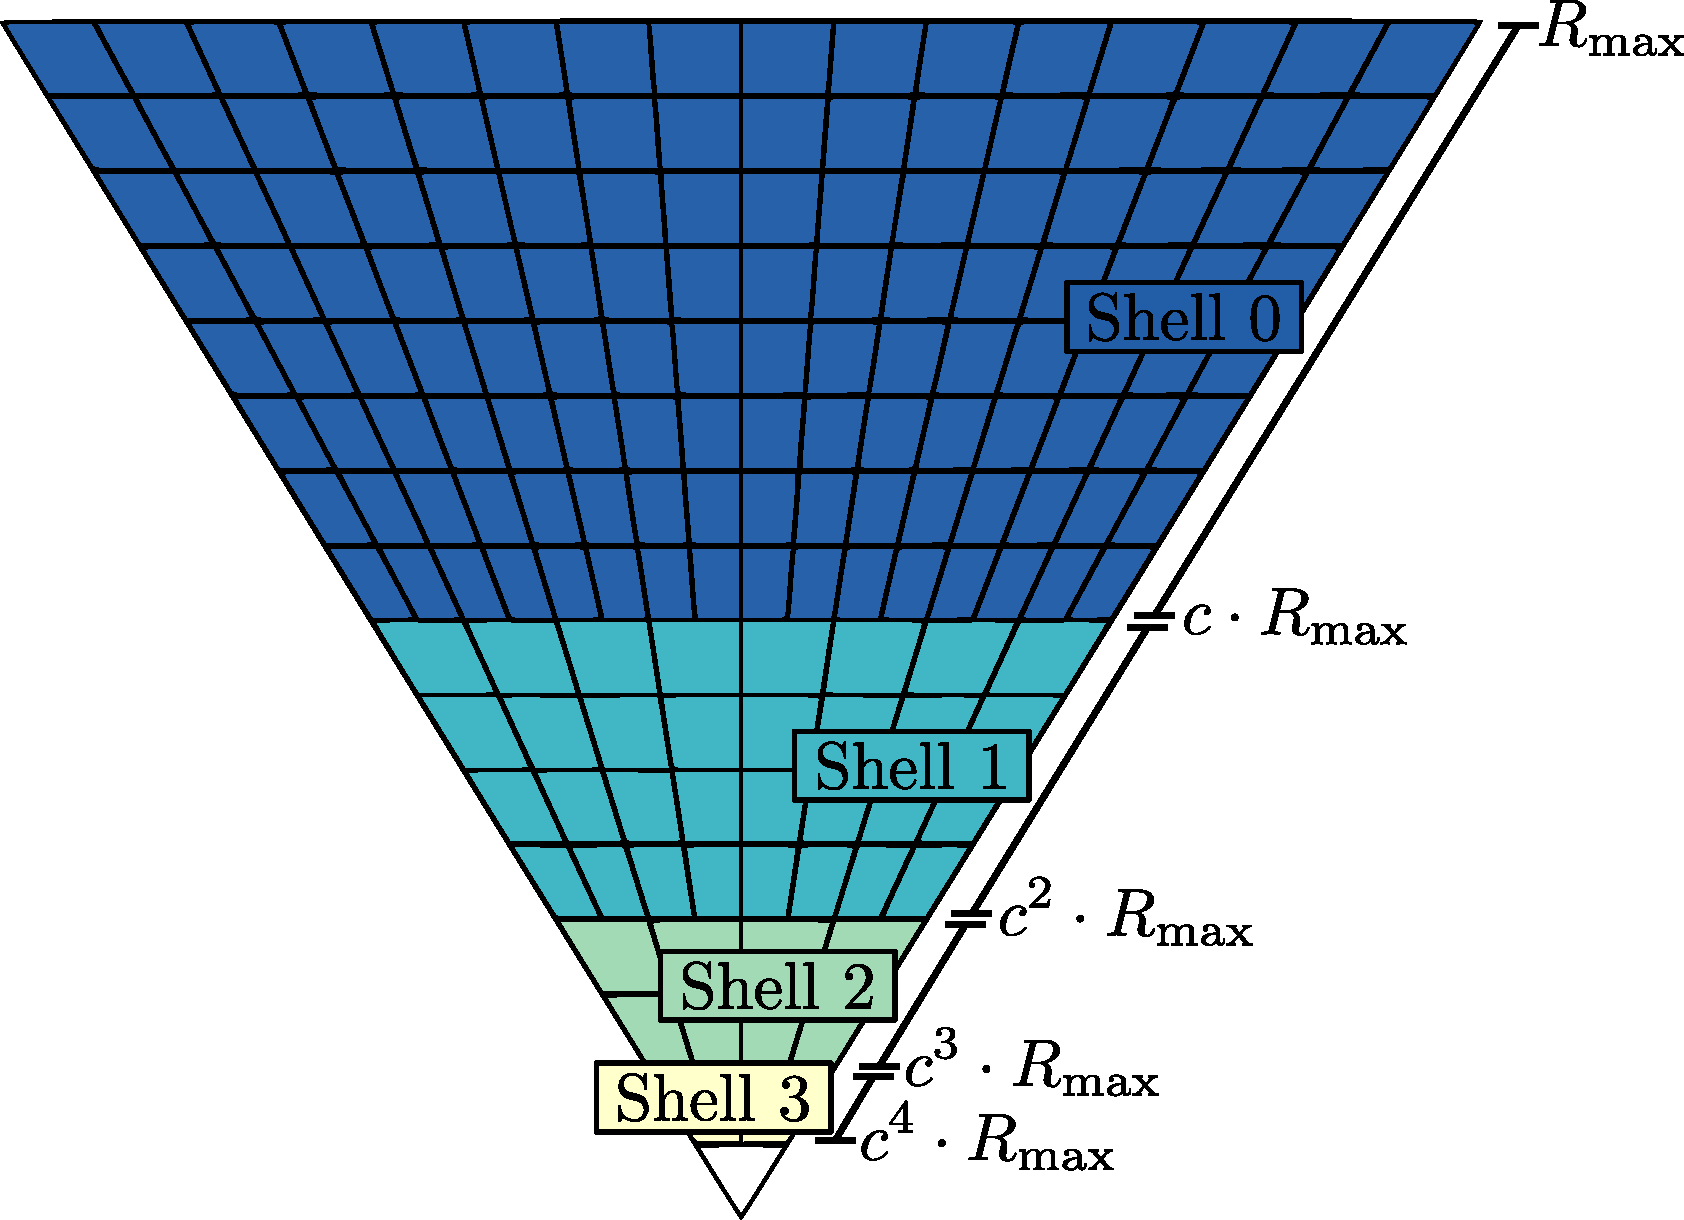
\includegraphics[width=0.675\textwidth]{prismatoid-shells.pdf}
	\caption[Spherical shells that result from the grid extension method]{
		Radial splits of central layers divide the grid into regions that represent spherical shells.
		At $k$ levels of refinement there are $k$ shells and the central layer.
		These shells are similar and should have a mapped volume proportional to the number of cells they contain
	}
	\label{fig:prismatoid-shells}
\end{figure}


Radii at powers of $1/2$ in the grid should be mapped to corresponding powers of $\alpha$ in physical domain.
For a given $\hat{r}$ then, need to find one above and one below.
Shell $s = \lfloor \log_{0.5} \hat{r} \rfloor$.
Can then find these splits in both grid and physical domain by raising to appropriate power.
%
\begin{equation*}
\ell_p = \alpha^{s + 1}, \quad u_p = \alpha^s, \quad \ell_g = 0.5^{s + 1}, \quad \text{and} \quad u_g = 0.5^s.
\end{equation*}
%
Mapping can be achieved then by finding a percent between $\ell_g$ and $u_g$ and then mapping said percent between $\ell_p$ and $u_p$.
Call percent $d$, then
%
\begin{equation} \label{eq:radialInvD}
d = \frac{ \hat{r} - \ell_g }{ u_g - \ell_g }
\end{equation}
%
How $d$ is interpolated between $\ell_p$ and $u_p$ affects volume preservation.
Using a linear interpolation is the same as conventional SDOG and latitude method, cubic is the volume method, and a power of $t$ gives the balanced method.
Thus, the general formulation is
%
\begin{equation} \label{eq:radialInv}
M_r^{-1}(\hat{r}) = \sqrt[t]{ d u_p^{t} + \left( 1 - d \right) \ell_p^{t} }
\end{equation}
%
which is just a more general form of Equation~radialblend.


From this we can derive the forward mapping by inverting the inverse.
Can solve Equation~\ref{eq:radialInv} for $d$ to get
%
\begin{equation} \label{radialForwD}
d = \frac{ \hat{r}^{\,t} - \ell_p^{\,t} }{ u_p^{\,t} - \ell_p^{\,t} }
\end{equation}
%
and solve Equation~\ref{eq:radialInvD} for $\hat{r}$ to get
%
\begin{equation} \label{eq:radialForw}
M_r (\hat{r}) = d u_g + \left( 1 - d \right) \ell_g
\end{equation}
%
Uppers and lowers are the calculated the same, but the shell is now $s = \lfloor \log_{c} \hat{r} \rfloor$.


The results of this mapping for different values of $t$ applied to the grid extension method are shown in Figure~X. These mappings have the side effect of changing the aspect ratio of cells in grid space as compared to in physical space. This means that when determining the refinement parameters needed to achieve the desired aspect ratio, the cells in physical space should be considered as opposed to grid space.
This is accomplished by setting the value of $\nu$ in Equations~X and X to be $(1 - \alpha)$.


\section{Latitude Mappings for SDOG} \label{chap:6:latitude}
Goal is to define function $M_\varphi(\varphi)$. Consider latitude to be normalized with $\hat{\varphi} = (2\varphi) / \pi$.


Follows same general principles as radial mapping.
Zones go in opposite direction as shells in parameter space.
At 1 - powers of 0.5 as opposed to powers themselves.
So then zone $z = \lfloor \log_{0.5} ( 1 - \hat{\varphi} ) \rfloor$.
We then calculate uppers and lowers just as with radial mapping, but accounting for opposite direction
%
\begin{equation*}
\ell_p = 1 - 0.25^{z}, \quad u_p = 1 - 0.25^{z + 1}, \quad \ell_g = 1 - 0.5^z, \quad \text{and} \quad u_g = 1 - 0.5^{z + 1}.
\end{equation*}
%
Remember, these are in parameter domain, not angles themselves. Get angles with inverse sin.
Mapping can be achieved then by finding a percent between $\ell_g$ and $u_g$ and then mapping said percent between $\ell_p$ and $u_p$.
Call percent $d$, then
%
\begin{equation} \label{eq:latInvD}
d = \frac{ \hat{\varphi} - \ell_g }{ u_g - \ell_g }
\end{equation}
%
How $d$ is interpolated between $\ell_p$ and $u_p$ affects volume preservation.
Using a linear interpolation is the same as conventional SDOG and latitude method, sin is the volume method, and a scaled sin by $h$ gives the balanced method.
Thus, the general formulation is
%
\begin{equation} \label{eq:latInv}
M_\varphi^{-1}(\hat{\varphi}) = h \arcsin \left( d \sin \left( \frac{1}{h} \arcsin u_p \right) + \left( 1 - d \right) \sin \left( \frac{1}{h} \arcsin \ell_p \right) \right)
\end{equation}
%
This simplifies to
%
\begin{equation*}
M_\varphi^{-1}(\hat{\varphi}) = d \arcsin u_p  + \left( 1 - d \right) \arcsin \ell_p
\end{equation*}
%
for the latitude method as $h \rightarrow \infty$ and
%
\begin{equation*}
M_\varphi^{-1}(\hat{\varphi}) = \arcsin \left( d u_p + \left( 1 - d \right) \ell_p \right)
\end{equation*}
%
for the volume method when $h = 1$.
Volume is efficient (one arcsin), latitude is moderately efficient (two arcsin), and balanced is worst (three arcsin, two sin).


From this we can derive the forward mapping by inverting the inverse.
Can solve Equation~\ref{eq:latInv} for $d$ to get
%
\begin{equation} \label{latForwD}
d = \frac{ \sin \left( \frac{1}{h} \hat{\varphi} \right) - \sin \left( \frac{1}{h} \arcsin \ell_p \right) }{ \sin \left( \frac{1}{h} \arcsin u_p \right) - \sin \left( \frac{1}{h} \arcsin \ell_p \right) }
\end{equation}
%
and solve Equation~\ref{eq:latInvD} for $\hat{\varphi}$ to get
%
\begin{equation} \label{eq:latForw}
M_\varphi (\hat{\varphi}) = d u_g + \left( 1 - d \right) \ell_g
\end{equation}
%
Uppers and lowers are the calculated the same, but the zone is now $z = \lfloor \log_{0.25} ( 1 - \sin \hat{\varphi} ) \rfloor$.
Once again, Equation~\ref{latForwD} simplifies to
%
\begin{equation*}
d = \frac{ \hat{\varphi} - \arcsin \ell_p }{ \arcsin u_p - \arcsin \ell_p}
\end{equation*}
%
for the latitude method as $h \rightarrow \infty$ and
%
\begin{equation*}
d = \frac{ \sin \hat{\varphi} - \ell_p }{ u_p - \ell_p }
\end{equation*}
%
for the volume method when $h = 1$.
Once again, volume is efficient (one sin), latitude is moderately efficient (three arcsin), and balances is worst (three arcsin, four sin).


\section{Summary}
Provide mappings for use with modified SDOG grids and extension method.
For SDOG, mapping go between the modified grids and conventional SDOG.
This allows efficient algorithms defined on regular midpoint SDOG to be used with modified grids.
For extension, allows same volume preserving properties (in radial dimension) of modified SDOG grids to be applied to grid extension method.
Mapping are all closed form and constant time (no iterative solves) for both forward and inverse.
Efficiency varies significantly for latitude depending on which scheme.
Balanced method particularly bad; this is result of function chosen in Chapter~\ref{chap:sdog}.
A different function could help alleviate this, however we could not find one that met other needed properties as well.
